\documentclass[oneside, final, 14pt]{extreport}
\usepackage[utf8]{inputenc}
\usepackage[russian]{babel}
\usepackage{vmargin}
\setpapersize{A4}
\setmarginsrb{2cm}{1cm}{1cm}{1cm}{0pt}{0mm}{0pt}{13mm}
\usepackage{indentfirst}
\usepackage{amsmath}
\usepackage{graphicx}
\usepackage{wrapfig}
\sloppy

\begin{document}

\setcounter{chapter}{4}
\chapter{Шумоподавление}
\section{Основные понятия}

Целью шумоподавления и восстановления звука является получение наилучшего звучания с минимальным вмешательством человека. По сути, редактирование исходной записи должно быть незаметным и не создавать новые артефакты, которые бы отвлекали слушателя.

Шумоподавление применяется, для того, чтобы:
\begin{itemize}
  \item улучшить восприятие сигнала, в том числе различимость речи;
  \item удалить искажения, наводки от сети электрического тока из записей музыки;
  \item упростить сведение мультитрековых композиций (например, уменьшив количество низкочастотных составляющих сигнала).
\end{itemize}

Иногда целей шумоподавления можно достичь в полном объеме, иногда приходится искать компромисс между уменьшением шумов и сохранением оригинального звучания.

\textit{Шумом} может считаться любой нежелательный звук, присутствующий в аудио сигнале, например:
\begin{itemize}
\item шипение усилителя;
\item шум уличного движения;
\item наводки от сети переменного тока;
\item периодические щелчки на оцифрованной записи виниловой пластинки.
\end{itemize}

\textit{Искажение}~--– это нежелательное изменение формы сигнала. Примеры искажений:
\begin{itemize}
\item клипирование;
\item нелинейные искажения звукового сигнала, полученные при прохождении через усилитель c нелинейным коэффициентом передачи.
\end{itemize}

Некоторые искажения можно обнаружить при анализе спектрограммы, обращая внимание на области, яркость которых выделяется по сравнению с яркостью близлежащих областей (например, на рис. \ref{pic-distort-01} более яркие области с непрерывным спектром рядом с тонами в средних частотах).

\begin{figure}[h]
\centering
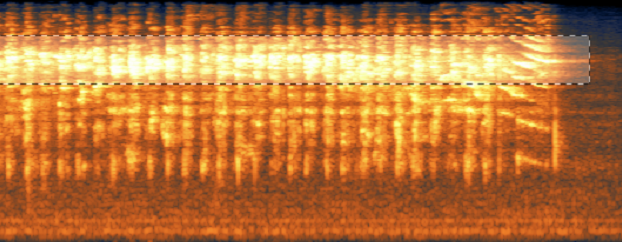
\includegraphics[width=0.75\textwidth]{pic-distort-01}
\caption{Пример спектрограммы сигнала с искажением}
\label{pic-distort-01}
\end{figure}

Инструменты для шумоподавления и восстановления звука можно разделить на следующие группы:
\begin{itemize}
\item \textbf{Шумоподавители} (\textit{Denoisers}) используются для того, чтобы уменьшить или полностью удалить постоянный фоновый шум. Это может быть фоновый шум помещения или шипение магнитофонной ленты (примеры "<случайных"> шумов), либо электрическое жужжание или гул от сети переменного тока (примеры "<тональных"> шумов). Шумоподавители могут быть одно- и многополосными, программными (\textit{Audition Noise Reduction}) и аппаратными (\textit{iZotope ANR-B}), общего применения или разработанными для особых задач, например, обработке вокала.
\item \textbf{Инструменты удаления щелчков} (\textit{Declickers}) используются, чтобы уменьшить или удалить щелчки и хлопки. Причина их появления может быть разной: грязь и царапины на оцифровываемой виниловой пластинке,  скачки луча лазера при захвате данных с аудио компакт-диска, а также звуки причмокивания и размыкания губ.
\item \textbf{Инструменты удаления треска} (\textit{Decracklers}) похожи на инструменты удаления щелчков, но оптимизированы для уменьшения или удаления более продолжительных и более тихих последовательных щелчков, которые, соединяясь воспринимаются нашим ухом как треск.
\item \textbf{Инструменты удаления клипирования} (\textit{Declippers}) используются для восстановления артефактов цифрового и/или аналогового клипирования.
\item \textbf{Инструменты удаления реверберации} (\emph{Dereverbs}) предназначены для удаления из сигнала нежелательной и отвлекающей реверберации. Эти инструменты полезны для коррекции диалогов, в том числе при \emph{ADR} (\emph{Automatic Dialog Replacement}~--- автоматическая замена диалога).
\item \textbf{Инструменты визуального ручного редактирования сигнала} (\emph{Visual Editing Tools}) представляют собой комбинированные средства отображения и редактирования сигнала в различных формах: сигналлограммы и спектрограммы, в том числе средства позволяющие выделить и отредактировать как определенный диапазон (во времени и частоте), так и сигнал целиком.
\end{itemize}

В данной лекции будут рассмотрены следующие инструменты шумоподавления:
\begin{itemize}
  \item стандартные инструменты подавления шума в \emph{Adobe Audition}, за исключением средств, которые представляют собой варианты фильтров, эквалайзеров и инструментов динамической обработки (они будут рассмотрены в соответствующих лекциях);
  \item некоторые средства из набора VST-инструментов, входящих в пакет \emph{Waves Restoration bundle};
  \item инструмент \emph{iZotope RX 3 Advanced}, который может использоваться и как VST-инструмент, и как отдельное приложение \emph{Win x86/x64};
\end{itemize}

\section{Устранение непериодических шумов}

Вне зависимости, какое программное обеспечение будет использовано для устранения непериодических шумов, для восстановления звука и шумоподавления обязательно будут использоваться инструменты визуального редактирования. Практически всегда редактирование будет происходить в режиме отображения спектрограммы, так как это позволяет производить точное выделение требуемых областей спектра сигнала. Затем выделенные области могут быть заменены (или использоваться как шаблон для замены), либо подвергнуты восстановлению. Качественное программное обеспечение, как правило, содержит целый ряд различных инструментов выделения определенных областей спектра.

После того, как требуемая область на спектрограмме выделена, производится обработка сигнала,~--- применяются необходимые инструменты шумоподавления. В любом случае, необходимо ясно и четко представлять задачи и последствия своих действий по корректировке спектра.

Удаление непериодических шумов может представлять некоторые трудности, так как:
\begin{itemize}
  \item такие шумы могут вести себя непредсказуемо как по частоте, так и во времени;
  \item в отличие от нетональных шумов, гула, щелчков и треска, такие шумы нельзя удалить с использованием автоматических методов, а ручная коррекция может быть довольно трудоемкой;
  \item даже самые современные инструменты могут создать артефакты в сигнале в результате процесса шумоподавления;
  \item всегда существует множество разнообразных инструментов, подходящих для решения конкретной задачи по подавлению шума, а выбор наиболее эффективного средства тоже непростая задача.
\end{itemize}

\subsection{Устранение непериодических шумов в \emph{Adobe Audition}}
В \textit{Adobe Audition} в режиме отображения спектрограммы можно использовать следующие инструменты для того, чтобы выделить звук в определенном частотном диапазоне:
\begin{itemize}
\item \textit{Marquee Selection}~--– выделение прямоугольной области,
\item \textit{Lasso Selection}~--– выделение при помощи лассо,
\item \textit{Paintbrush Selection}~--– эффект кисти.
\end{itemize}

\begin{figure}[h]
\centering
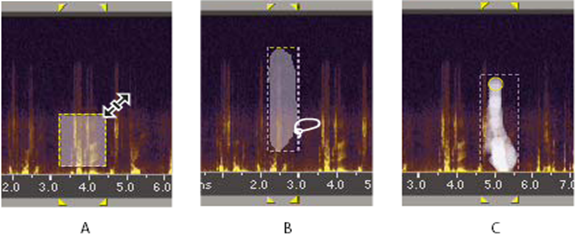
\includegraphics[width=0.75\textwidth]{pic-spectroedit-01}
\caption{Инструменты выделения области спектрограммы}
\label{pic-spectroedit-01}
\end{figure}

Эффект \textit{Paintbrush} позволяет создавать выделенные области, которые задают мощность применения эффектов (задаются параметром \textit{Size} (размер кисти) и \textit{Opacity }(непрозрачность) на панели инструментов). Чем ближе цвет выделенной области к белому цвету, тем сильнее будет применен эффект.

Для быстрого исправления небольших дискретных искажений, таких как отдельные хлопки и щелчки, следует использовать инструмент \textit{Spot Healing Brush}.
Для использования данного средства следует выполнить следующие действия:
\begin{itemize}
\item в режиме \textit{Spectral Frequency Display} выбрать инструмент \textit{Spot Healing Brush};
\item на панели инструментов установить размер кисти (\textit{Brush Si}ze).
\item в главном окне щелкнуть или провести мышью по области искажения.
\end{itemize}

\begin{figure}[h]
\centering
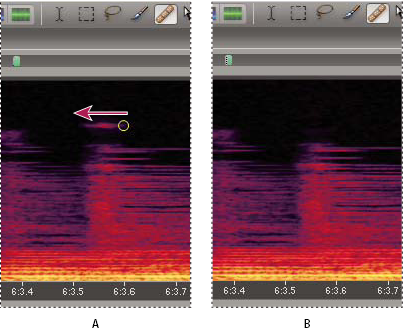
\includegraphics[width=0.5\textwidth]{pic-spectroedit-02}
\caption{Применение эффекта \textit{Spot Healing Brush}}
\label{pic-spectroedit-02}
\end{figure}

В режиме отображения спектрограммы категорически не рекомендуется корректировать низкочастотные составляющие сигнала, так как исправление может затронуть основные гармоники речи.

\subsection{Устранение непериодических шумов в \emph{iZotope~RX~3}}
Инструмент \emph{iZotope~RX~3}~--- это полноценный инструмент для проведения шумоподавления и восстановления звука, который может использоваться и как VST-инструмент, и как отдельное приложение \emph{Win x86/x64}.

Основные инструменты и их возможности в \emph{iZotope~RX~3}:
\begin{itemize}
  \item \emph{Denoise, Remove Hum}~--- удаление фонового шума и шумов и искажений сигнала, в том числе шипение, гул и жужжание;
  \item \emph{Spectral Repair}~---замена поврежденных или отсутствующих фрагментов сигнала с использованием шаблонов на основе естественных звуков;
  \item \emph{DeClick, DeCrackle}~--- удаление щелчков, хлопков;
  \item \emph{DeClip}~---избавление от клипирования.
\end{itemize}

\begin{figure}[h]
\centering
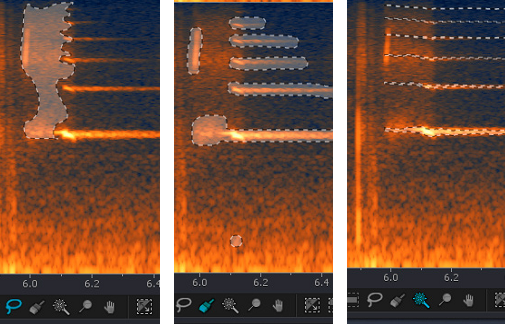
\includegraphics[width=0.5\textwidth]{pic-spectroedit-03}
\caption{Инструменты выделения областей на спектрограмме в iZotope~RX~3}
\label{pic-spectroedit-03}
\end{figure}

Для редактирования и применения эффектов, в том числе шумоподавления, необходимо выделять определенные области на спектрограмме. В \emph{iZotope~RX~3} имеются следующие инструменты:

\begin{itemize}
  \item \emph{Time Selection}~--- выделение временного интервала спектрограммы;
  \item \emph{Time-Frequency Selection}~--- выделение прямоугольного фрагмента спектрограммы;
  \item \emph{Frequency Selection}~--- выделение диапазона частот на спектрограмме;
  \item \emph{Lasso}~--- позволяет нарисовать произвольный замкнутый контур на спектрограмме.
  \item \emph{Brush}~--- выделение "<кистью">;
  \item \emph{Magic Wand}~--- "<волшебная палочка">, автоматическое "<умное"> выделение некоторого диапазона на спектрограмме.
\end{itemize}

После выделения фрагмента, подлежащего корректировке, следует выбрать инструмент \emph{Spectral Repair}. Данный инструмент позволяет восстановить звучание выделенного фрагмента (который считается поврежденным) на основе информации из близлежащих к выделенной областей.

Фрагмент сигнала выделен при помощи инструмента \emph{Time Selection}, то при помощи инструмента \emph{Spectral Repair} можно получить лучший результат по сравнению с инструментом \emph{Declick} для фрагментов (длительностью до 10 мс).

Если фрагмент выделен при помощи любого другого инструмента, то при помощи инструмента \emph{Spectral Repair} можно удалить (или уменьшить)
нежелательные составляющие сигнала, такие, как скрип стула, кашель, сопение, свист, шумы падения объектов, стук микрофонной стойки, звонки мобильного телефона, звук метронома, щелчки, звуки дверей, вздохи, смех, цифровые артефакты, ошибки из-за отключения кабелей и т.д.

Кроме того, при помощи \emph{Spectral Repair} можно восстанавливать пропуски в сигнале (см. рис. \ref{pic-repair-02}) с использованием технологии ресинтеза звука.

Существуют следующие режимы для восстановления сигнала:
\begin{itemize}
  \item \emph{Attenuate} (ослабление)~--- в этом режиме звук в выделенном фрагменте заменяется звуками, расположенными в близлежащих областях. Данный режим бывает полезен для записей с фоновым шумом или записей, в которых шум~--- составная часть музыки (например, ударные или перкуссия), следовательно, необходима аккуратная обработка, чтобы не повредить звук; либо, когда шумы не занимают диапазон полезного сигнала целиком.
  \item \emph{Replace} (замена)~--- данный режим используется для замены поврежденных фрагментов тонального сигнала. Выделенный фрагмент целиком заменяется результатом интерполяции значений из близлежащих областей.
  \item \emph{Pattern} (шаблон)~--- в данном режиме ищется наиболее подходящий фрагмент сигнала, которым и заменяется выделенный фрагмент. Данный режим полезен для сильно поврежденных записей с фоновым шумом или для записей, имеющих повторяющиеся фрагменты.
  \item \emph{Partials + Noise}~--- это более сложный вариант режима \emph{Pattern}, выполняющий более точную интерполяцию в тех случаях, когда происходит изменение высоты тона, в том числе в виде вибрато.
\end{itemize}

\begin{figure}[h]
  \centering
  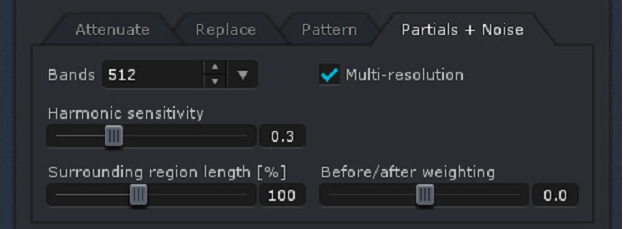
\includegraphics[width=0.5\textwidth]{pic-repair-01}
  \caption{Окно \emph{Spectral Repair}, вкладка \emph{Partials + Noise}}
  \label{pic-repair-01}
\end{figure}

\begin{figure}[h]
  \centering
  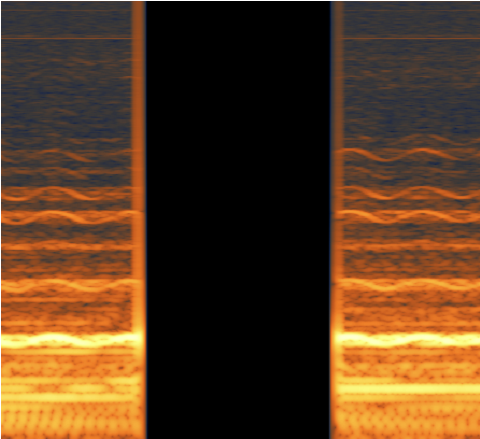
\includegraphics[width=0.5\textwidth]{pic-repair-02}
  \caption{Спектрограмма сигнала c пропуском в 1/2 секунды, вибрато и изменением высоты тона}
  \label{pic-repair-02}
\end{figure}

Рассмотрим основные параметры окна \emph{Spectral Repair}:

\begin{itemize}
  \item \emph{Number of bands}~--- количество частотных полос, используемых при интерполяции. Чем больше значение данного параметра, тем больше точность, но и тем больше требуется окружающего пространства вокруг выделенного фрагмента.
  \item при включенном флажке \emph{Multi-Resolution} для низких и высоких частот будет использовано большее число частотных полос.
  \item параметр \emph{Surrounding region} задает размер области, окружающей выделенный фрагмент, которая будет использоваться при интерполяции.
  \item параметр \emph{Before/after weighting} задает соотношение весовых коэффициентов интерполяции для областей до и после выделенного фрагмента.
  \item параметр \emph{Direction} для режиме \emph{Attenuate} задает направление, из которого будет выбран фрагмент для восстановления записи.
  \item параметр \emph{Strength} изменяет величину ослабления в режиме \emph{Attenuate}.
  \item параметр \emph{Pattern Search Range} задает интервал в секундах для поиска подходящего фрагмента для замены в режиме \emph{Pattern}.
  \item параметр \emph{Harmonics sensitivity} изменяет количество обнаруживаемых гармоник в режиме \emph{Partials + Noise}. Чем меньше значение данного параметра, тем меньше гармоник будет обнаружено, при больших значениях могут появляться неестественные изменения высоты тона звука.
\end{itemize}


\section{Устранение нетональных шумов}
Для удаления нетональных шумов необходимо иметь информацию о шуме: чем больше статистических свойств шума известно, тем эффективнее процесс шумоподавления.

Информацию о шуме можно получить, анализируя спектр фрагмента волновой формы, содержащий только шумы (шипение микрофона, фоновые звуки и т. п.). При выполнении процесса шумоподавления будет считаться, что выбранный фрагмент содержит только шум.

\begin{figure}[h]
\centering
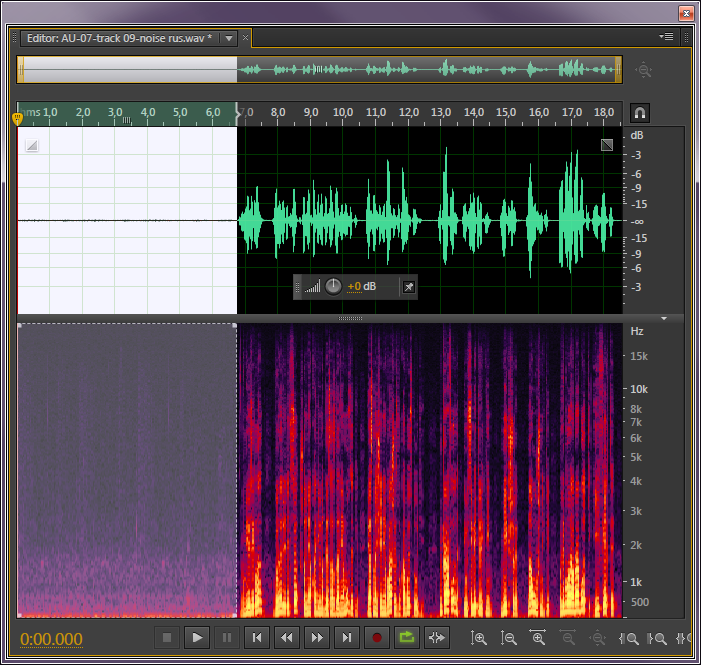
\includegraphics[width=0.5\textwidth]{pic-noisereduction-01}
\caption{Выделение фрагмента сигнала, содержащего шум}
\label{pic-noisereduction-01}
\end{figure}

\subsection{Устранение нетональных шумов в Adobe Audition}
Рассмотрим процесс шумоподавления при помощи инструмента \textit{Noise Reduction}.
\begin{enumerate}
    \item Прежде чем вызывать окно шумоподавления, необходимо в главном окне программы выделить фрагмент волновой формы без полезной информации, но содержащий характерный для этой волновой формы шум. Желательно, чтобы этот фрагмент был как можно длиннее (рис. \ref{pic-noisereduction-01}).
    \item Выполнить команду \textit{Effects > Restoration > Noise Reduction}. В открывшемся окне нажать кнопку "<\emph{Capture Noise Print}">. Запустится процесс анализа спектра выделенного фрагмента, который отобразится в верхнем координатном поле.
    \item На координатном поле отображаются три графика:
        \begin{itemize}
            \item красный: минимально возможный уровень шумоподавления;
            \item желтый: максимально возможный уровень шумоподавления;
            \item зеленый: текущий уровень шумоподавления. Величина этого параметра регулируется параметром \textit{Noise Reduction}.
        \end{itemize}
        \begin{figure}[h]
            \centering
            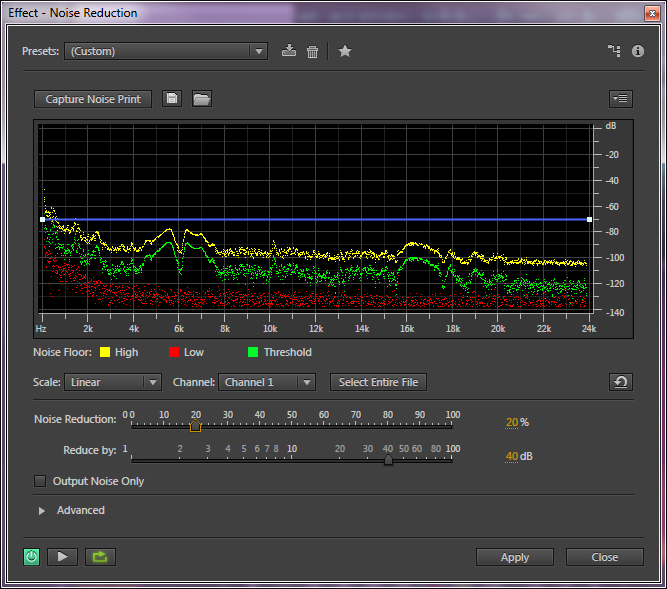
\includegraphics[width=0.5\textwidth]{pic-noisereduction-02}
            \caption{Окно инструмента \textit{Noise reduction}}
            \label{pic-noisereduction-02}
        \end{figure}
    \item Характеристики шума можно сохранить в файле, воспользовавшись кнопкой \textit{Save the current noise print}. Теперь, если в будущем вы захотите очистить от шума аудио файл, записанный в той же шумовой обстановке, нужно будет нажать кнопку \textit{Load a noise print from disk} и загрузить соответствующий файл с характеристиками шума (и не выполнять расчет профиля шума повторно).
    \item Снять флаг \textit{Output Noise Only} (выводить только шум), если он был установлен. Нажать на кнопку "\textit{Preview Play/Stop}". Прослушивая фрагмент с шумом, установить значение параметра \textit{Noise Reduction}, при котором шум становится практически не слышен (абсолютной тишины добиваться не следует). Если выбрать порог подавления слишком высоким, то улучшения субъективного ощущения тишины в паузах не будет, зато в сигнале появятся искажения в виде металлического призвука.
    \item Установить флаг \textit{Output Noise Only}. Прослушивая звук и уменьшая значение \textit{Noise Reduction}, добиться, чтобы не удалялись полезные составляющие звука (то есть при прослушивании не были бы слышны отдельные гласные, согласные звуки и т.п.).
    \item Попеременно выполняя пункт 5 и пункт 6 установить компромиссное значение параметра \textit{Noise Reduction}, чтобы, с одной стороны, обеспечивать достаточный уровень шумоподавления, а с другой~--– не затрагивать полезный сигнал.
\end{enumerate}

\subsection{Устранение нетональных шумов в \emph{Waves X-Noise} и \emph{Waves Z-Noise}}
Инструмент \emph{Waves X-Noise} (рис. \ref{pic-xnoise-01}) также предназначен для удаления фонового шума. В отличие от инструмента \textit{Adobe Audition Noise Reduction}, инструмент \emph{X-Noise} может быть использован в режиме реального времени после предварительной настройки профиля шума.

\begin{figure}[h]
    \centering
    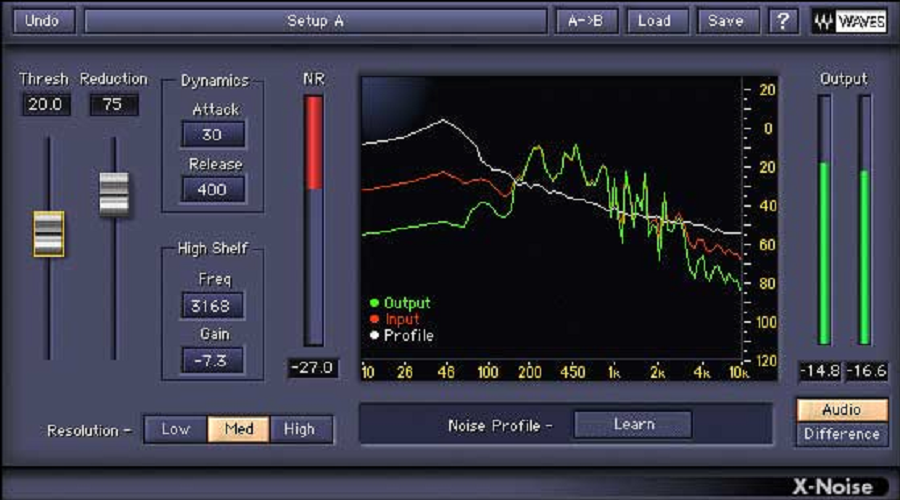
\includegraphics[width=0.5\textwidth]{pic-xnoise-01}
    \caption{Окно инструмента \textit{Waves X-Noise}}
    \label{pic-xnoise-01}
\end{figure}

Рассмотрим основные этапы использования инструмента \emph{Waves X-Noise}.

\begin{enumerate}
  \item \emph{Создание профиля шума}. Для создания профиля шума следует выделить фрагмент сигнала, содержащего только шум и нажать на кнопку \textbf{Learn}. Запустится процесс анализа частотного состава шума. Для того, чтобы этот процесс остановить, следует повторно нажать на кнопку \textbf{Learn}. После этого в окне отобразиться спектр шума (линия белого цвета).
  \item \emph{Шумоподавление}. После создания профиля шума следует снять выделение фрагмента сигнала, для того, чтобы работать с сигналом целиком. При воспроизведении следует выполнять подбор параметров:
      \begin{itemize}
        \item \textbf{Threshold} (порог)~--- задает уровень профиля шума (для разделения шума и полезного сигнала). Сигнал, расположенный ниже профиля шума будет обработан, выше~--- нет.
        \item \textbf{Reduction} (ослабление)~--- задает количество удаляемого шума (в процентах).
      \end{itemize}
      Если в процессе воспроизведения слышны артефакты (например, голос приобретает металлическое звучание), то следует настраивать параметры \textbf{Attack} (время атаки), \textbf{Release} (время восстановления), \textbf{Resolution} (сложность алгоритма шумоподавления) и \textbf{High Shelf} (изменение профиля шума на высоких частотах).
  \item Мониторинг процесса шумоподавления следует проводить, переключаясь между обработанным сигналом (режим \textbf{Audio}) и удаляемым шумом (режим \textbf{Difference}). При мониторинге следует обращать внимание и на графики спектра (рис. \ref{pic-xnoise-02}):
      \begin{itemize}
        \item красный график~--- спектр входного сигнала;
        \item белый график~--- профиль шума;
        \item зеленый график~--- спектр выходного сигнала.
      \end{itemize}
\end{enumerate}

\begin{figure}[h]
    \centering
    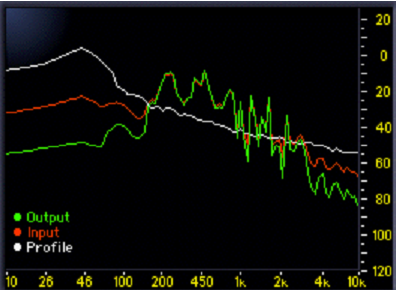
\includegraphics[width=0.5\textwidth]{pic-xnoise-02}
    \caption{Отображение графика спектра исходного, обработанного сигнала и профиля шума}
    \label{pic-xnoise-02}
\end{figure}

Инструмент \emph{Waves Z-Noise} (рис. \ref{pic-znoise-01}) отличается от \emph{Waves X-Noise} возможностью более точной настройки профиля шума. В распоряжении пользователя имеется пятиполосный параметрический эквалайзер, позволяющий вручную корректировать профиль шума.

Кроме того, имеется режим \textbf{Adaptive}: в этом режиме алгоритм шумоподавления может учитывать изменение характеристик шума с течением времени.

\begin{figure}[h]
    \centering
    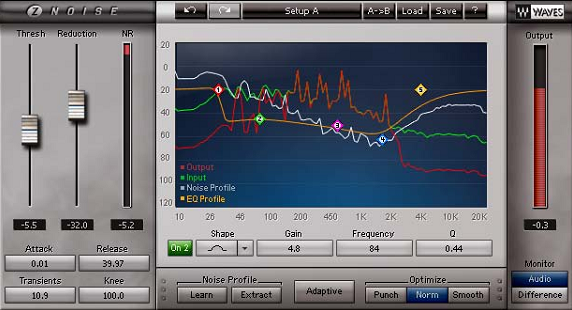
\includegraphics[width=0.5\textwidth]{pic-znoise-01}
    \caption{Окно инструмента \textit{Waves Z-Noise}}
    \label{pic-znoise-01}
\end{figure}

\subsection{Устранение нетональных шумов в \emph{iZotope RX3 Denoise}}
Инструмент \emph{iZotope Denoise} (рис. \ref{pic-rx3denoise-01}) также предназначен для шумоподавления на основе профиля шума. Рассмотрим отличия данного инструмента от ранее описанных:
\begin{itemize}
  \item возможность выделения не связанных областей для получения профиля шума;
  \item возможность раздельного управления уровнем подавления случайных и тональных шумов (\emph{Noisy, Tonal Reduction});
  \item возможность управления качеством обработки (параметр \emph{Quality}) и уровнем вносимых искажений (параметр \emph{Artifact Control}).
\end{itemize}

\begin{figure}[h]
    \centering
    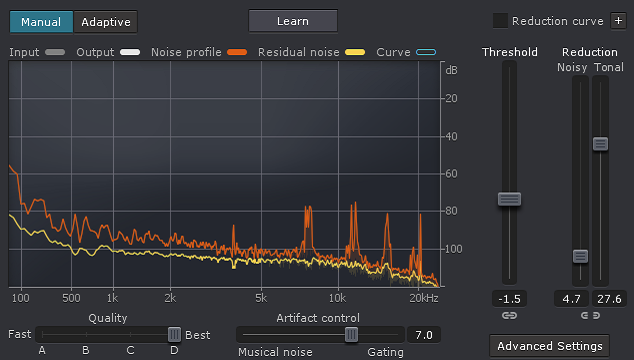
\includegraphics[width=0.5\textwidth]{pic-rx3denoise-01}
    \caption{Окно инструмента \textit{iZotope RX3 Denoise}}
    \label{pic-rx3denoise-01}
\end{figure}

\section{Устранение щелчков и треска}
Щелчки и хлопки могут оказаться в записи сигнала на любой стадии его обработки. Рассмотрим различные причины их возникновения:
\begin{itemize}
  \item цифровые ошибки, которые создают быстрые резкие перепады в амплитуде сигнале;
  \item ошибки, возникшие из-за повреждения носителя аналогового сигнала (как правило, это более длительные искажения по сравнению с цифровыми);
  \item статическое электричество;
  \item касание микрофона по неосторожности;
  \item плохой контакт соединительных кабелей;
  \item помехи от электрической сети;
  \item звуки размыкания губ и т.д.
\end{itemize}

Для того чтобы найти щелчки на волновой форме, следует переключиться в режим отображения \textit{Spectral Frequency Display}. Большинство щелчков будут видны как вертикальные линии, яркие на всей полосе частот.

\begin{figure}[h]
\centering
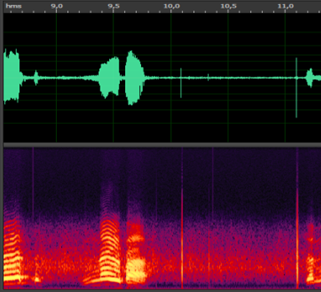
\includegraphics[width=0.5\textwidth]{pic-click-01}
\caption{Пример сигналограммы и спектрограммы сигнала с щелчками}
\label{pic-click-01}
\end{figure}

В зависимости от типа щелчка, он может иметь некоторые отличия на спектрограмме. На рис. \ref{pic-click-05} в верхней части представлена спектрограмма записи с щелчками, которые возникают при воспроизведении виниловой пластинки, в нижней~--- спектрограмма помех от сотового телефона.

В первом случае спектр щелчка непрерывен, а сам щелчок может считаться случайным. Во втором случае при увеличении масштаба (см. рис. \ref{pic-click-06} ) можно рассмотреть, что на самом деле эта помеха является очень коротким периодическим сигналом.

\begin{figure}[h]
\centering
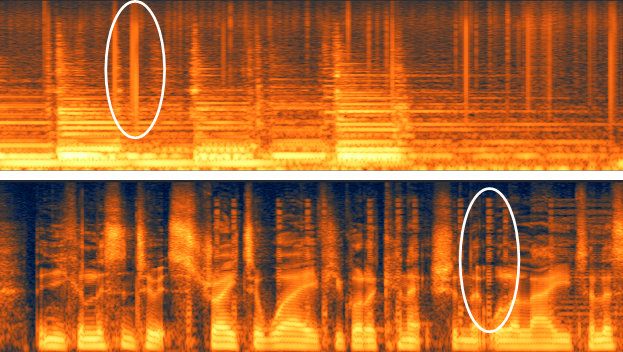
\includegraphics[width=0.5\textwidth]{pic-click-05}
\caption{Пример спектрограммы сигнала с щелчками}
\label{pic-click-05}
\end{figure}

\begin{figure}[h]
\centering
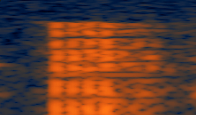
\includegraphics[width=0.35\textwidth]{pic-click-06}
\caption{Пример спектрограммы сигнала с помехами от сотового телефона}
\label{pic-click-06}
\end{figure}

Инструменты для устранения щелчков, как правило, имеют настройки для идентификации щелчков и для определения того, какие из них будут обработаны.

\subsection{Adobe Audition > DeClicker}
Средства \textit{Diagnostics > DeClicker} и \textit{Noise Reduction \& Restoration > Automatic Click Remover} позволяют определить и удалить такие искажения, как щелчки и хлопки.

Рассмотрим параметры эффекта \textit{Automatic Click Remover} (рис. \ref{pic-click-02}) .

\begin{figure}[h]
\centering
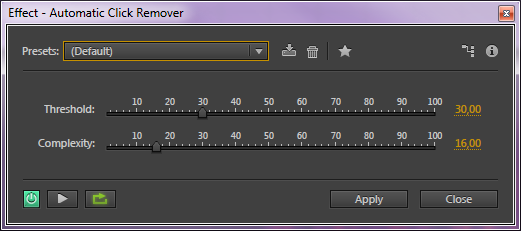
\includegraphics[width=0.5\textwidth]{pic-click-02}
\caption{Окно эффекта \textit{Automatic Click Remover}}
\label{pic-click-02}
\end{figure}

Параметр \textit{Threshold} (порог) определяет чувствительность к шуму. Уменьшение параметра позволяет обнаружить больше хлопков и щелчков, но может захватить звук, который вы желали бы сохранить. Параметр \textit{Complexity} (сложность) позволяет задать сложность обработки. Увеличение параметра увеличивает обработку звука, но может ухудшить качество звука.

\begin{figure}[h]
\centering
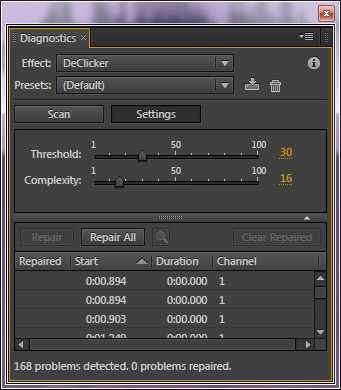
\includegraphics[width=0.5\textwidth]{pic-click-03}
\caption{Окно эффекта \textit{Diagnostics > DeClicker}}
\label{pic-click-03}
\end{figure}

\subsection{Waves > X-Click}
Инструмент \emph{X-Click} позволяет эффективно устранять щелчки старых виниловых пластинок и при правильном применении не создает дополнительных артефактов~--- искажений, вносимых эффектом. Инструмент \emph{X-Click} имеет два параметра настройки для идентификации щелчков:
\begin{itemize}
  \item Параметр \textbf{порог} (\textit{Threshold}) задает амплитуду искомых щелчков. Чем больше значение данного параметра, тем больше щелчков будет найдено; при значении  0 щелчки не будут найдены вообще. Для наиболее типичной оцифрованной записи виниловой пластинки рекомендуемое значение параметра \emph{Threshold}~$=30..50$.
  \item Параметр \textbf{форма} (\textit{Shape}) задает количество отсчетов в одном щелчке. Для цифровых щелчков следует задавать небольшие значения, для щелчков виниловой пластинки ориентировочное значение около $70$.
\end{itemize}

\begin{figure}[h]
\centering
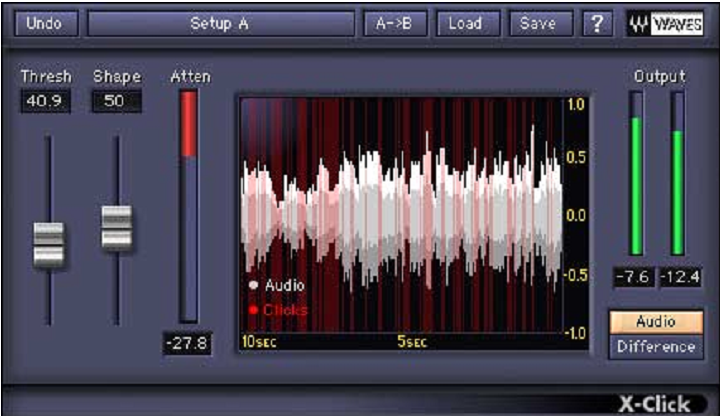
\includegraphics[width=0.5\textwidth]{pic-click-04}
\caption{Окно эффекта \textit{X-Click}}
\label{pic-click-04}
\end{figure}

При увеличении обоих параметров будут увеличиваться и артефакты, таким образом, необходимо искать компромисс между эффективностью удаления щелчков и качеством итогового сигнала.

Найденные щелчки для заданного параметра \textit{Treshold} отображаются в окне \textit{Click Scope} в виде линий красного цвета. Рекомендуется, изменяя значения параметров, одновременно осуществлять мониторинг сигнала.

Дополнительным средством мониторинга является переключатель \textit{Audio/Difference}, который в режиме \textit{Audio} позволяет прослушивать обработанный сигнал, а в режиме \textit{Difference}~--- только удаляемые в результате обработки щелчки. В режиме \textit{Difference} в идеальном случае должны быть слышны только щелчки, и не должны быть слышны части полезного сигнала. Если это не так, необходимо уменьшить параметр \textit{Threshold} и/или \textit{Shape}.

Когда сигнал содержит резкие перепады амплитуды, являющиеся полезной составляющей (например, звуки ударных инструментов и перкусcию), инструмент автоматической коррекции щелчков может удалить некоторые их них. Если не удается достичь баланса между удалением щелчков и сохранением качества звучания записи в целом, то щелчки необходимо исправлять вручную.

\subsection{Waves > X-Crackle}
Инструмент \emph{X-Crackle} позволяет уменьшить треск~--- особый вид шума в сигнале.

\textbf{Треск} (\emph{Crackle})~--- небольшие по амплитуде, короткие по длительности (несколько отсчетов) щелчки или хлопки, в большом количестве присутствующие в сигнале. Щелчки выражены более явно, чем треск, и часто имеют большую амплитуду, чем полезный сигнал. Несмотря на то, что треск менее заметен, он может звучать довольно раздражающим.

При восстановлении записей виниловых пластиной данный инструмент рекомендуется применять после инструмента \emph{X-Click}.

\emph{X-Crackle} (рис. \ref{pic-crackle-01}) имеет два параметра настройки для идентификации треска:
\begin{itemize}
  \item \textbf{Порог} (\emph{Threshold}) определяет амплитуду звука, который будет идентифицироваться как треск. Рекомендуемые значения параметра от 50 до 70. Чем запись больше зашумлена, тем больше рекомендуется устанавливать значение данного параметра.
  \item \textbf{Ослабление} (\emph{Reduction}) задает, на сколько децибел будут ослаблен обнаруженный треск.
\end{itemize}

В окне \emph{X-Scope} отображается удаленный шум в виде сигналограммы и спектрограммы. Прослушивая запись, следует определить, стоит ли подбирать параметры \emph{Threshold} и \emph{Reduction} так, чтобы обработать запись целиком и автоматически, либо оставить часть треска для ручной обработки.

\begin{figure}[h]
\centering
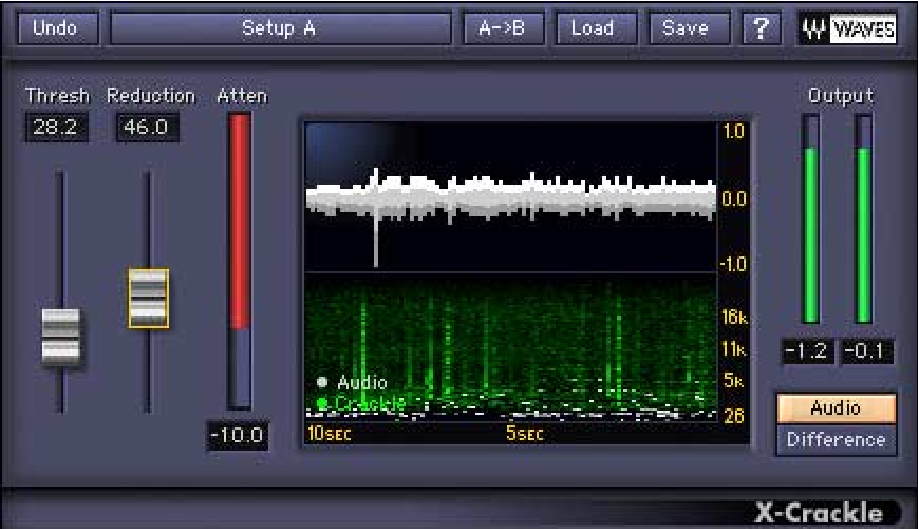
\includegraphics[width=0.5\textwidth]{pic-crackle-01}
\caption{Окно эффекта \textit{X-Crackle}}
\label{pic-crackle-01}
\end{figure}

Как и в предыдущем эффекте, имеется возможность прослушивать как обработанный сигнал, так и удаляемый из сигнала шум.

\subsection{iZotope Ozone > Declick \& Decrackle}

Инструмент \emph{Declick} полезен при восстановлении звука оцифрованных виниловых пластинок, избавления от таких шумов, как щелчки, хлопки и треск. Как правило, длительность отдельного щелчка не превышает 10 миллисекунд. Инструмент \emph{Decrackle} предназначен для удаления более длительных помех в сигнале, воспринимаемые нами как слабый треск.

На рисунке \ref{pic-rx3declick-01} представленная спектрограммы сигнала до и после удаления щелчков, а на рисунке \ref{pic-rx3declick-02} ~--- до и после удаления треска.

\begin{figure}[ht!]
\centering
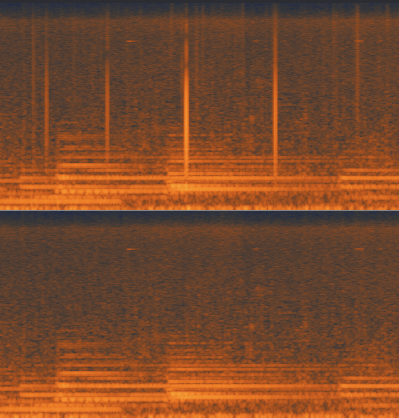
\includegraphics[width=0.5\textwidth]{pic-rx3declick-01}
\caption{Спектрограмма до и после удаления щелчков}
\label{pic-rx3declick-01}
\end{figure}

\begin{figure}[ht!]
\centering
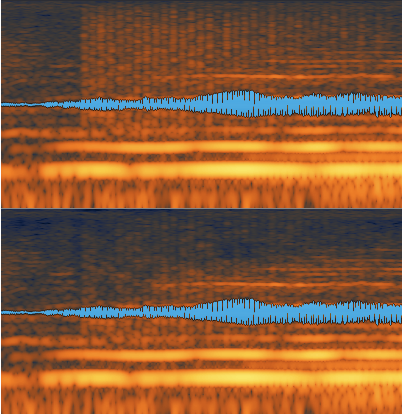
\includegraphics[width=0.5\textwidth]{pic-rx3declick-02}
\caption{Спектрограмма до и после удаления треска}
\label{pic-rx3declick-02}
\end{figure}

Для удаление щелчков и треска необходимо выполнить следующие шаги.
\begin{enumerate}
  \item Выберите нужное значение параметра \emph{Algorithm} для модуля \emph{Declick}:
  \begin{itemize}
    \item Режим \emph{Single-band} хорошо работает с очень короткими "<цифровыми"> щелчками.
    \item Ремим \emph{M-band} (\emph{multi-band}) предназначен для более длительных "<аналоговых"> щелчков.
  \end{itemize}
  \item Воспроизведите сигнал.
  \item Во время воспроизведения настройте параметр \emph{Declick Sensitivity}, задающий чувствительность детектора щелчков или \emph{Decrackle Strength} для чувствительности детектора треска. Необходимо добиться того, что большинство щелчков будет удалено, при этом полезный сигнал не будет повреждаться.
  \item Для лучшего контроля за тем, какие звуки идентифицируются как щелчки и треск, можно использовать переключатель \emph{Clicks/Crackle Only} во время воспроизведения сигнала,~--- это позволит  услышать, какие звуки будут удалены из сигнала.
\end{enumerate}

\begin{figure}[h]
\centering
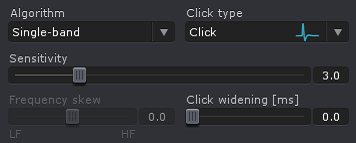
\includegraphics[width=0.5\textwidth]{pic-rx3declick-03}
\caption{Окно инструмента \emph{Declick}}
\label{pic-rx3declick-03}
\end{figure}

\begin{figure}[h]
\centering
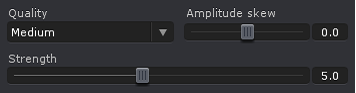
\includegraphics[width=0.5\textwidth]{pic-rx3decrackle-01}
\caption{Окно инструмента \emph{Decrackle}}
\label{pic-rx3decrackle-01}
\end{figure}

\section{Устранение клипирования}
\textit{Клипирование}~--- это искажение, возникающее из-за неправильной регулировки уровня записываемого сигнала или из-за его случайного увеличения во время записи, приведшее к переполнению разрядной сетки аналого-цифрового преобразователя (рис. \ref{pic-clip-01}).

Данное искажение можно обнаружить по результатам визуального анализа волновой формы~--- на сигналограмме могут быть фрагменты с прямой горизонтальной огибающей. По результатам статистического анализа обнаружить клипирование бывает не всегда возможно, так как после клипирования сигнала его громкость могла быть понижена, и в результате отсчеты формально не будут клипированы.

Чисто технически исправить клипирование можно и вручную, изменяя положение отдельных отсчетов вручную. Инструменты устранения клипирования используют автоматические интеллектуальные технологии для восстановления клипированного сигнала.

\begin{figure}[h!]
\centering
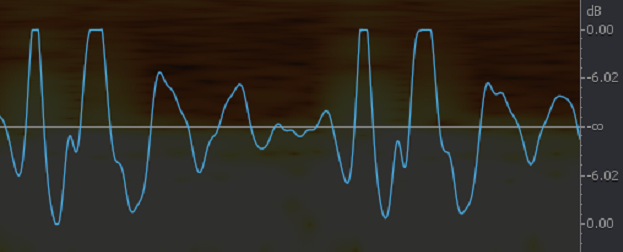
\includegraphics[width=0.5\textwidth]{pic-clip-01}
\caption{Сигналограмма с клипированием}
\label{pic-clip-01}
\end{figure}

Целью удаления клипирования является восстановление клипированых фрагментов сигнала таким образом, чтобы их звучание было бы наиболее близко к оригинальному (рис. \ref{pic-clip-02}). Нельзя избавиться от клипирования, просто уменьшив громкость: формально клипированных отсчетов не будет, но само искажение останется.

\begin{figure}[h!]
\centering
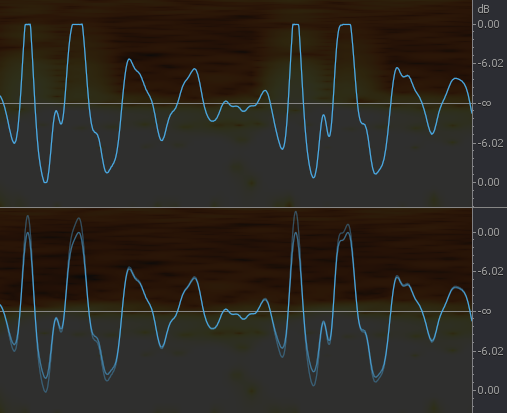
\includegraphics[width=0.5\textwidth]{pic-clip-02}
\caption{Сигналограмма с клипированием и результат ее обработки}
\label{pic-clip-02}
\end{figure}

В некоторых случаях избавиться от клипирования невозможно: например, старые фонограммы, которые были неоднократно перезаписаны, могут иметь иметь искажения от износа носителей аналогового сигнала (т.н. \emph{groove wall distortion}).

\subsection{Применение инструмента \emph{Adobe Audition DeClipper}}
\textit{Adobe Audition DeClipper} вызывается командой \textit{Effects > Diagnostics > DeClipper} (см. рис. \ref{pic-declipper-01}).

Параметр \emph{Gain}~--— усиление (фактически~--– ослабление, так как значения только отрицательные) сигнала перед обработкой. От этого параметра будет зависеть общая громкость звучания аудио файла после обработки.

\begin{figure}[ht!]
\centering
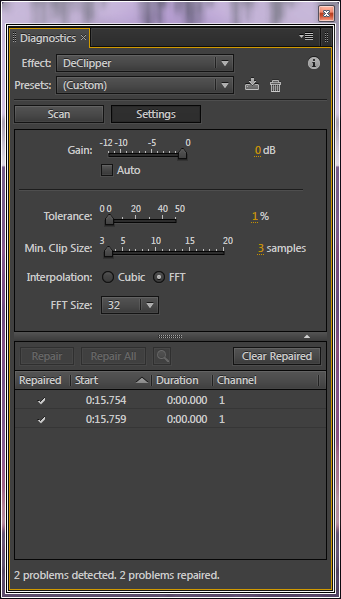
\includegraphics[width=0.3\textwidth]{pic-declipper-01}
\caption{Окно инструмента \textit{Diagnostics/DeClipper}}
\label{pic-declipper-01}
\end{figure}

Алгоритм избавления от клипирования следующий:
\begin{itemize}
\item установить значение параметра \textit{Gain} вручную или установить флаг \textit{Auto};
\item нажать кнопку \textit{Scan};
\item нажать кнопку \textit{Repair All}.
\end{itemize}

\subsection{Применение инструмента \emph{iZotope~RX~3 Declip}}

Инструмент \emph{Declip} (рис. \ref{pic-rx3declip-01}) производит обработку части сигнала, которая окажется выше задаваемого порога, выполняя интерполяцию сигнала с целью получения более натуральной огибающей. Процесс работы с инструментом состоит из двух простых шагов:

\begin{itemize}
  \item поиск клипированных отсчетов;
  \item определение уровня клипированных отсчетов и выполнение обработки.
\end{itemize}

\begin{figure}[h!]
\centering
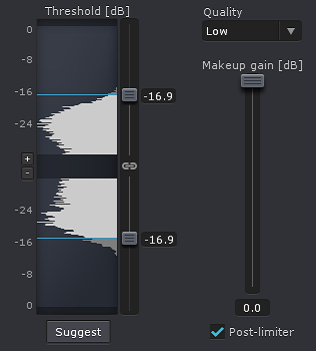
\includegraphics[width=0.4\textwidth]{pic-rx3declip-01}
\caption{Окно инструмента \textit{iZotope~RX~3 Declip}}
\label{pic-rx3declip-01}
\end{figure}

Левую часть окна занимает гистограмма сигнала, при этом установить порог клипирования можно независимо для положительных и отрицательных значений отсчетов. Одним из признаков наличия клипирования является наличие максимумов на гистограмме на уровнях, близких к максимальному уровню сигнала (рис. \ref{pic-rx3declip-02}):

\begin{figure}[h!t]
\centering
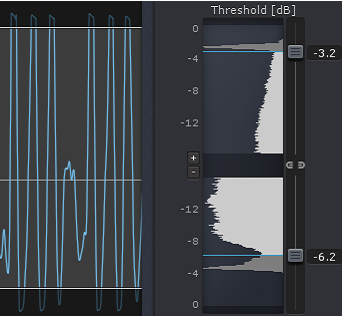
\includegraphics[width=0.4\textwidth]{pic-rx3declip-02}
\caption{Пример гистограммы с клипированием}
\label{pic-rx3declip-02}
\end{figure}

Для устранения клипирования необходима настройка следующих параметров:
\begin{itemize}
  \item \emph{Threshold (dBFS)}~--- задает уровень, относительно которого будет осуществляться поиск клипированных фрагментов сигнала. Данному параметру следует установить значение, чуть ниже уровня клипированных отсчетов;
  \item \emph{Threshold Link}~--- переключатель, позволяющий задавать различное значение порога для положительных и отрицательных значений отсчетов. Это может потребоваться в том случае, если клипирование имеется только в одной из двух областей: положительной или отрицательной (рис. \ref{pic-rx3declip-03}) и обработка второй области нежелательна;
\begin{figure}[h!]
  \centering
  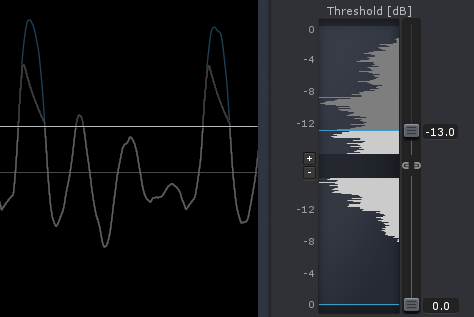
\includegraphics[width=0.4\textwidth]{pic-rx3declip-03}
  \caption{Пример гистограммы с двумя различными порогами клипирования}
  \label{pic-rx3declip-03}
\end{figure}
  \item кнопка \emph{Suggest} для автоматической установки значения параметра \emph{Threshold};
  \item \emph{Quality}~--- позволяет выбрать один из трех вариантов сложности работы алгоритма: легкий, средний или сложный.
  \item \emph{Makeup Gain (dB)}~--- величина ослабления или усиления сигнала после его обработка.
  \item \emph{Post-limiter}~--- применять ли лимитер с порогом 0 dBFS к обработанному сигналу.
\end{itemize}

\section{Устранение реверберации при помощи \emph{iZotope RX 3 Dereverb}}
Инструмент \emph{Dereverb} (рис. \ref{pic-rx3dereverb-01}) позволяет задавать уменьшать уровень реверберации в сигнале. При помощи данного инструмента запись, сделанную в большом помещении с сильном эхо можно как бы превратить в запись, сделанную в обычной комнате, а запись в комнате~--- в запись в помещении со звукоизоляцией.

\begin{figure}[h!]
  \centering
  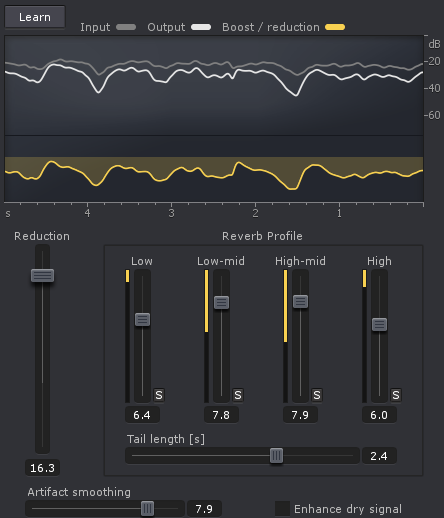
\includegraphics[width=0.5\textwidth]{pic-rx3dereverb-01}
  \caption{Окно инструмента \emph{iZotope RX 3 Dereverb}}
  \label{pic-rx3dereverb-01}
\end{figure}

Звук, записанный в помещении, можно разложить на две составляющих:
\begin{itemize}
  \item прямой звук;
  \item реверберационный хвост;
\end{itemize}

Уровень хвоста реверберации ослабляется с течением времени, причем скорость ослабления зависит от различных факторов, таких, как размер и материал стен помещения, его геометрия и т.д.

Инструмент \emph{Dereverb} выполняет обработку сигнала, изменяя соотношение обнаруженного прямого звука, и заданных (рассчитанных) параметров реверберации, таких как время ослабления сигнала на различных частотах.

На спектрограмме наличие реверберации можно обнаружить по наличию некоторой размытости. На рисунке \ref{pic-rx3dereverb-02} представлены примеры спектрограмм сигнала с реверберацией (приемник звука располагался далеко от источника звука) и результаты обработки по уменьшению хвоста реверберации (по центру, первый проход) и уменьшению ранних отражений (справа, второй проход).

\begin{figure}[h!]
  \centering
  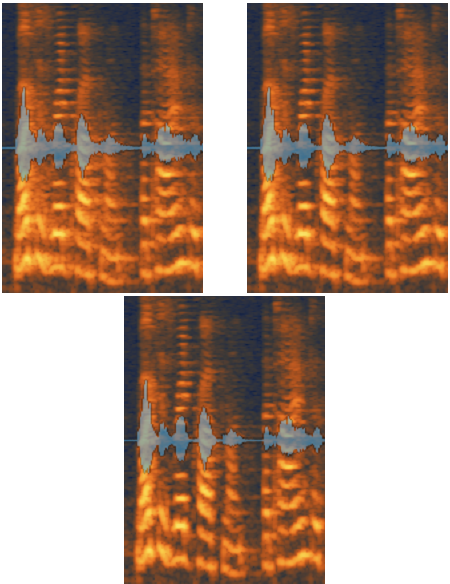
\includegraphics[width=0.5\textwidth]{pic-rx3dereverb-02}
  \caption{Пример спектрограммы с реверберацией (слева), результатом удаления реверберации (по центру) и ранних отражений (справа)}
  \label{pic-rx3dereverb-02}
\end{figure}

Для того, чтобы приступить к уменьшению реверберации в сигнале, необходимо получить так называемый "<профиль реверберации">. Для этого необходимо выделить фрагмент сигнала, длительностью около 5 секунд, который будет содержать фоновый шум помещения в начале, полезный сигнал и хвост реверберации.

После получения профиля реверберации (после нажатия на кнопку \textit{Learn}) в верхней части окна отобразятся графики входного, выходного сигнала и величина ослабления (частотная характеристика профиля реверберации). Управлять процессом удаления реверберации можно при помощи следующих параметров:
\begin{itemize}
  \item \emph{Reduction}~--- величина ослабления реверберации (при отрицательных значениях~--- усиление).
  \item \emph{Reverb Profile}~--- элементы управления профилем реверберации на разных частотных полосах для более точного подбора параметров реверберации.
  \item \emph{Tail Length}~--- величина хвоста ревеберации. Если реверберация проявляется после обработки сигнала, то следует увеличивать значение данного параметра.
  \item \emph{Artifact Smoothing}~--- сглаживание артефактов, управляет точностью обработки сигнала.
  \item \emph{Enhance Signal}~--- увеличивает уровень прямого звука.
\end{itemize}

Иногда хороших результатов удается достичь, применяя инструмент \emph{Dereverb} дважды. На первом этапе необходимо постараться удалить длинный реверберационный хвост, а на втором~--- заново получить профиль реверберации и задать \emph{Tail Length}$=0.5$, \emph{Artifact Smoothing} $=3.0$, и увеличить параметр \emph{Reduction}.

\section{Шумоподавление в записях диалогов при помощи \emph{iZotope RX 3 Dialog Denoiser}}
Инструмент \emph{Dialogue Denoiser} (рис. \ref{pic-rx3dialog-01}) позволяет осуществлять подавление шума в записях, в которых уровень шума значительно отличается от уровня полезного сигнала. Уровень шума задается при помощи графика порога шума. Если уровень сигнал ниже порога, то он считается шумом и будет подавляться, если выше ~--- полезным сигналом. Настройка формы графика порога шума осуществляется при помощи шести контрольных точек.

\begin{figure}[h!]
  \centering
  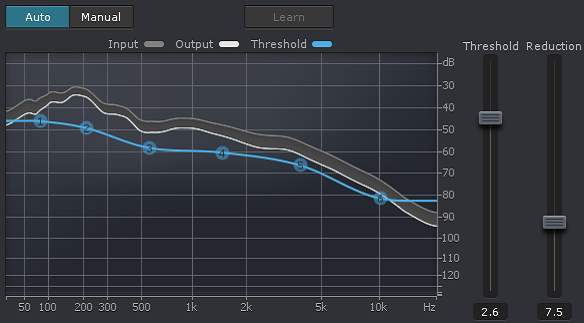
\includegraphics[width=0.4\textwidth]{pic-rx3dialog-01}
  \caption{Окно инструмента \emph{iZotope RX 3 Dialog Denoiser}}
  \label{pic-rx3dialog-01}
\end{figure}

В инструменте \emph{Dialogue Denoiser} реализована возможность автоматического расчета графика порога шума на основе анализа сигнала (режим \emph{Auto}). При ручном (\emph{Manual}) режиме сначала необходимо выделить фрагмент сигнала, содержащий шум и нажать кнопку \emph{Learn}.

Параметр \emph{Threshold} позволяет задавать общее для всех контрольных точек смещение (сдвигая, таким образом, график порог шума в целом). Чем больше значение данного параметра, тем в большей степени будет удален шум, однако при больших значениях из сигнала могут начать удаляться полезные низкие по громкости составляющие. Параметр \emph{Reduction} задает величину ослабления шума в децибелах.

\end{document}

